\documentclass[12pt,a4paper]{article}

\usepackage{fontspec}
\setmainfont{Times New Roman}
\setmonofont{Menlo}[Scale=0.80]
\usepackage[brazil]{babel}
\usepackage[a4paper,left=3cm,right=2cm,top=2.5cm,bottom=2cm]{geometry}
\usepackage{setspace}
\usepackage{graphicx}
\usepackage{float}
\usepackage{booktabs}
\usepackage{array}
\usepackage{caption}
\usepackage{titlesec}
\usepackage[hidelinks]{hyperref}

\titleformat{\section}{\normalfont\bfseries}{}{0pt}{}
\titlespacing*{\section}{0pt}{1.1\baselineskip}{0.4\baselineskip}
\captionsetup{labelsep=endash,font=small,justification=centering}
\newcommand{\code}[1]{\texttt{\detokenize{#1}}}
\setlength{\fboxsep}{1pt}
\setlength{\emergencystretch}{3em}
\setlength{\parindent}{1.25cm}

\begin{document}
\onehalfspacing

\begin{center}
{\footnotesize
PONTIFÍCIA UNIVERSIDADE CATÓLICA DO RIO GRANDE DO SUL — LABORATÓRIO DE REDES DE COMPUTADORES\par}
\vspace{0.4cm}
{\bfseries\large INTERCEPTAÇÃO E DEFESA DE UM PROTOCOLO DE APLICAÇÃO\par}
{\bfseries Fase 2: interceptação ativa (Man-in-the-Middle)\par}
\vspace{0.2cm}
{\footnotesize Bernardo Garcia \quad Gabriel Vieira \quad Guilherme Cavazzotto \quad — \quad Porto Alegre, 2026\par}
\end{center}
\vspace{0.3cm}

\section{Objetivo}

Posicionar um proxy entre o cliente e o servidor do protocolo KVP e mostrar que,
sem integridade nem autenticação, o conteúdo pode ser lido e alterado em
trânsito sem que as pontas percebam. O proxy atende várias sessões ao mesmo
tempo e resiste a desconexões e mensagens malformadas.

\section{Arquitetura do proxy MITM}

O proxy (\code{proxy/proxy_mitm.py}) aceita a conexão do cliente, abre a conexão
ao servidor real e faz o relay das mensagens nos dois sentidos. O
redirecionamento é por configuração: o cliente aponta o \code{--host} para o
proxy em vez do servidor, sem saber que fala com um intermediário.

Para cada mensagem (uma linha do KVP), o proxy inspeciona o conteúdo e aplica
regras de modificação antes de repassar. As duas regras usadas na demonstração:

\begin{itemize}\setlength{\itemsep}{0pt}
\item \textbf{C\,$\rightarrow$\,S:} troca o valor de \code{SET destino ...} por
      \code{conta-do-atacante} (adultera um comando que vai ao servidor).
\item \textbf{S\,$\rightarrow$\,C:} troca a resposta \code{VALUE saldo ...} por
      \code{VALUE saldo 999999} (adultera uma resposta que volta ao cliente).
\end{itemize}

\section{Concorrência e robustez}

O proxy usa uma thread por sessão e, dentro de cada sessão, duas threads de
relay (uma por sentido), pois cada sentido fica bloqueado em leitura e não pode
travar o outro. O estado compartilhado (contador de sessões, estatísticas e o
log) é protegido por locks; as regras de modificação são só leitura. Cada sessão
é isolada: uma desconexão ou uma linha malformada afeta apenas a própria sessão.
O detalhamento está em \code{docs/CONCORRENCIA.md}.

\section{Ambiente de teste}

A demonstração rodou em \textbf{nós isolados}, não em loopback. Três contêineres
com IPs distintos numa rede bridge \code{10.10.0.0/24}: cliente
(\code{10.10.0.30}), proxy (\code{10.10.0.20}) e servidor (\code{10.10.0.10}). O
tráfego entre eles passa por Ethernet real. O mesmo código roda igual em três
VMs separadas. Toda a evidência a seguir vem de \textbf{uma única execução}
(\code{deploy/run_demo.sh}), capturada nos dois trechos ao mesmo tempo.

\section{Evidência da modificação}

Capturamos os dois trechos da mesma sessão. A Tabela~\ref{tab:cmp} compara, nos
mesmos pacotes, o que passou de cada lado do proxy.

\begin{table}[H]
\centering
\caption{O mesmo pacote nos dois trechos: o proxy altera o conteúdo.}
\label{tab:cmp}
\small
\begin{tabular}{@{}c l l@{}}
\toprule
\textbf{Pacote} & \textbf{Trecho cliente$\leftrightarrow$proxy (.30$\leftrightarrow$.20)} & \textbf{Trecho proxy$\leftrightarrow$servidor (.20$\leftrightarrow$.10)} \\
\midrule
\#10 (C$\rightarrow$S) & \code{SET destino conta-do-bernardo} & \code{SET destino conta-do-atacante} \\
\#20 (S$\rightarrow$C) & \code{VALUE saldo 999999} & \code{VALUE saldo 100} \\
\bottomrule
\end{tabular}
\\[2pt]{\footnotesize Fonte: os autores (2026).}
\end{table}

As Figuras~\ref{fig:cli} e~\ref{fig:srv} mostram, no Wireshark, a mesma sessão
reconstruída (\emph{Follow TCP Stream}) nos dois trechos. No trecho do cliente
aparece o que o cliente enviou e recebeu; no trecho do servidor, o que o
servidor recebeu e enviou. A diferença entre as duas é a adulteração feita pelo
proxy.

\begin{figure}[H]
\centering
\caption{Trecho cliente$\leftrightarrow$proxy: o cliente envia \texttt{conta-do-bernardo} e recebe \texttt{saldo 999999}.}
\label{fig:cli}
\fbox{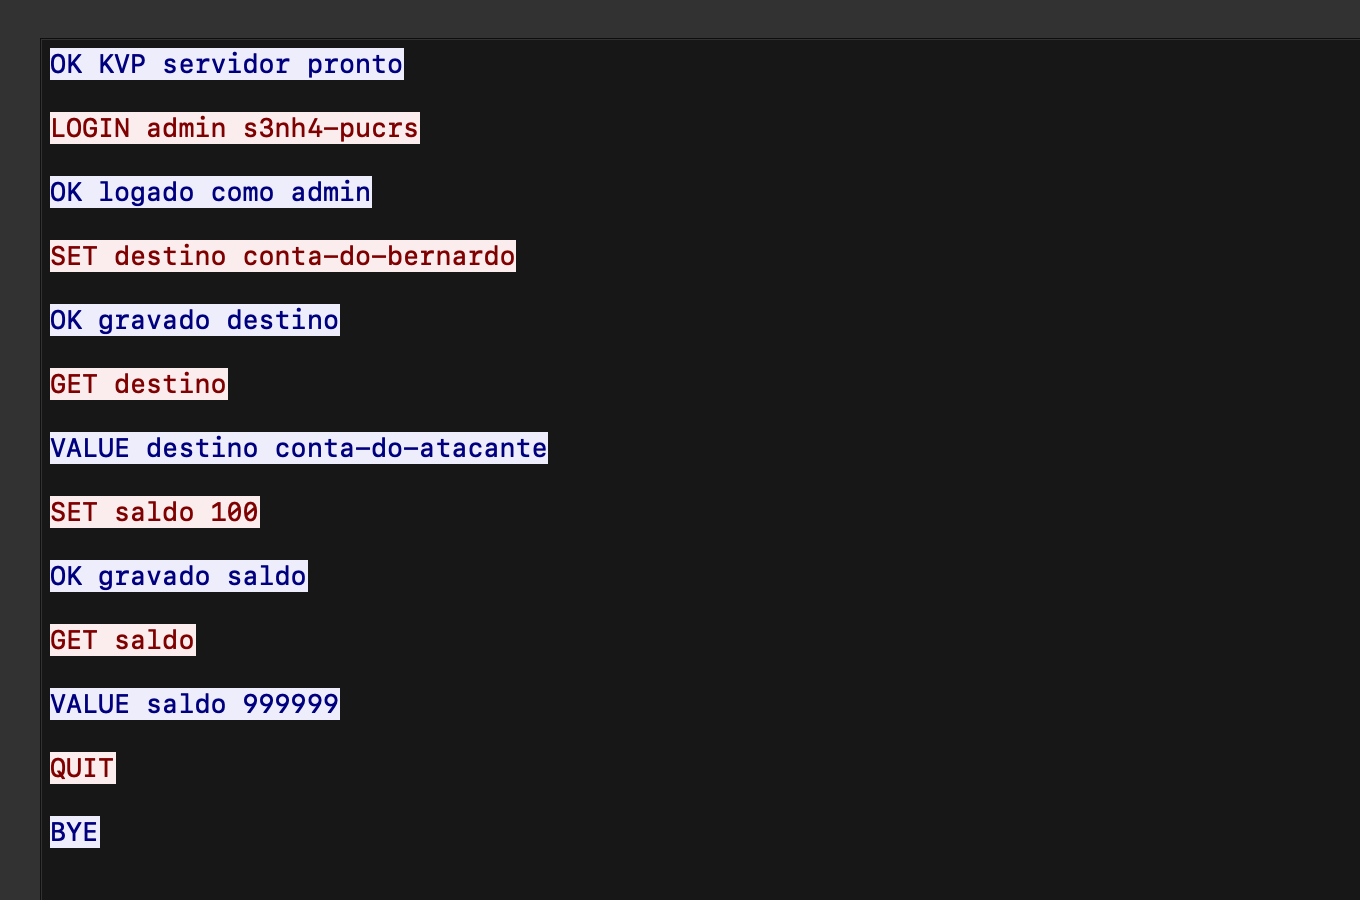
\includegraphics[width=0.86\linewidth]{capturas/fase2_fig_leg_cliente.png}}
\end{figure}

\begin{figure}[H]
\centering
\caption{Trecho proxy$\leftrightarrow$servidor: o servidor recebe \texttt{conta-do-atacante} e envia \texttt{saldo 100}.}
\label{fig:srv}
\fbox{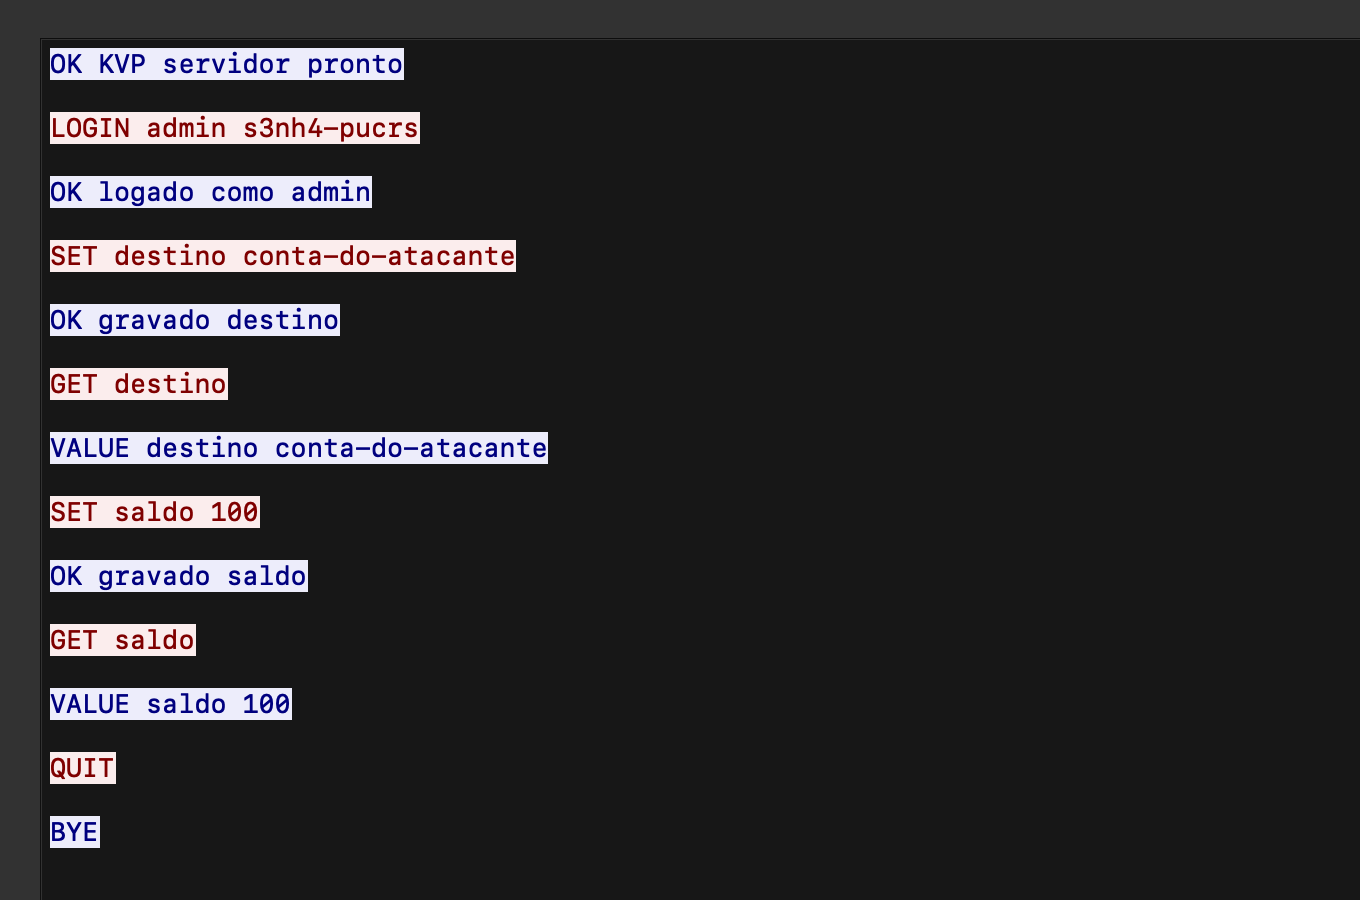
\includegraphics[width=0.86\linewidth]{capturas/fase2_fig_leg_servidor.png}}
\end{figure}

O log do proxy registra a leitura e a troca (sessão do cenário principal):

{\scriptsize
\begin{verbatim}
C->S ORIGINAL: SET destino conta-do-bernardo
C->S ALTERADA: SET destino conta-do-atacante   (regra_redireciona_destino)
S->C ORIGINAL: VALUE saldo 100
S->C ALTERADA: VALUE saldo 999999              (regra_infla_saldo)
\end{verbatim}
}

O servidor aceitou o comando adulterado como legítimo (gravou
\code{conta-do-atacante}) e o cliente aceitou a resposta adulterada como legítima
(leu \code{saldo 999999}). Nenhuma das pontas tem como detectar a troca.

\section{Concorrência e robustez (evidência)}

No mesmo experimento, três clientes passaram pelo proxy ao mesmo tempo. O log
mostra as sessões abertas simultaneamente antes de qualquer uma encerrar:

{\scriptsize
\begin{verbatim}
[sessao 4] nova conexao de 10.10.0.30:41926
[sessao 5] nova conexao de 10.10.0.30:41916
[sessao 6] nova conexao de 10.10.0.30:41938
[sessao 4] sessao encerrada
[sessao 5] sessao encerrada
[sessao 6] sessao encerrada
\end{verbatim}
}

Para a robustez, um cliente que enviou bytes inválidos e desconectou no meio
rodou em paralelo com um cliente normal; o normal concluiu sem ser afetado (ver
\code{fase2_robustez_cliente.txt} em \code{docs/capturas}).

\section{Conclusão}

O proxy MITM lê e altera as mensagens do KVP em trânsito, e as duas pontas
aceitam o conteúdo adulterado. Isso confirma a quebra de integridade e de
autenticação de um protocolo sem proteção. Na Fase 3, o canal receberá TLS
(para cifrar e garantir integridade) e autenticação do servidor por certificado,
o que impede o proxy de se passar pelo servidor e de alterar as mensagens sem
ser detectado.

\end{document}
